\documentclass[12pt, paper=a4]{article}
\usepackage[utf8]{inputenc}
\usepackage[german]{babel}
\usepackage{mathrsfs}
\usepackage{amsmath}
\usepackage{amssymb}
\usepackage{listings}
\usepackage{graphicx}
\usepackage{fancyhdr}

\setlength{\parindent}{0pt}

\author{Mareike G\"ottsch, 6695217, Gruppe 2\\Paul H\"olzen, 6673477, Gruppe 1\\Sven Schmidt, 6217064, Gruppe 1}

\title{FGI 2 Hausaufgaben 10}

\rhead{M. G\"ottsch, G-2; P. H\"olzen, G-1; S. Schmidt, G-1}
\pagestyle{fancy}
\begin{document}
\maketitle
\section*{10.3}

\subsection*{1.}
Die Wirkungsmatrix vom Netz \(N_{10.3}\) lautet:\\
\begin{center}
\begin{tabular}{ | c | c c c c c c | }
	\hline
	$\Delta_{N_{10.3}}$ & $a$ & $b$ & $c$ & $d$ & $e$ & $f$\\
	\hline
	$p1$ & -4 & 1 & -1 & 3 & 2 & -1\\
	$p2$ & 0 & 0 & -1 & 3 & 0 & 0\\
	$p3$ & 0 & 0 & 1 & -3 & 0 & 0\\
	$p4$ & 4 & -1 & 2 & -6 & -2 & 1\\
	\hline
\end{tabular}
\end{center}

Die Menge aller T-Invariantenvektoren ist die Menge der Vektoren $j^{tr} = (j_1 ... j_6) \in \mathbb{N}^6\backslash \{0\}$,
die das folgende Gleichungssystem \(\Delta_{N_{10.3}}(t) \cdot j = 0 \) l\"osen:\\

\begin{align*}
	&I) &-4\cdot j_1 + 1\cdot j_2 - 1\cdot j_3 + 3\cdot j_4 + 2\cdot j_5 - 1\cdot j_6 &= 0\\
	&II) &0\cdot j_1 + 0\cdot j_2 - 1\cdot j_3 + 3\cdot j_4 + 0\cdot j_5 + 0\cdot j_6 &= 0\\
	&III) &0\cdot j_1 + 0\cdot j_2 + 1\cdot j_3 - 3\cdot j_4 + 0\cdot j_5 + 0\cdot j_6 &= 0\\
	&IV) &+4\cdot j_1 - 1\cdot j_2 + 2\cdot j_3 - 6\cdot j_4 - 2\cdot j_5 + 1\cdot j_6 &= 0\\
\end{align*}

Offensichtlich sind die Gleichungen $II$ und $III$ linear abh\"angig, und f\"uhren zu gleichen L\"osungen, da \(j_i \in \mathbb{N}\) gilt f\"ur alle \(i \in \{1,...,6\}\). Setzt man eine der Gleichungen $II$ oder $III$ in $I$ oder $IV$ ein, so fallen die beiden mittleren Summanden weg und die Gleichungen $I$ und $IV$ sind auch linear abh\"angig.\\
Es ergibt sich also folgendes Gleichungssystem:\\
\begin{align*}
	&I') &-4\cdot j_1 + 1\cdot j_2 + 2\cdot j_5 - 1\cdot j_6 &= 0\\
	&II') & - 1\cdot j_3 + 3\cdot j_4 &= 0\\
\end{align*}
Alle Vektoren $j^{tr} = (j_1 ... j_6) \in \mathbb{N}^6\backslash \{0\}$ welche dieses LGS l\"osen sind also T-Invarianten vom Netz \(N_{10.3}\).

\subsection*{2.}
Es sei \(j = (1, 3, 3, 1, 1, 1)^{tr}\) einer der T-Invarianten-Vektoren. Au{\ss}erdem sei \(m_0 = (4, 3, 0, 0)^{tr}\).\\

\(m_0=\begin{pmatrix} 4\\ 3 \\ 0 \\ 0 \end{pmatrix} \underrightarrow{a} 
	\begin{pmatrix} 0\\ 3 \\ 0 \\ 4 \end{pmatrix} \underrightarrow{b}
	\begin{pmatrix} 1\\ 3 \\ 0 \\ 3 \end{pmatrix} \underrightarrow{b}
	\begin{pmatrix} 2\\ 3 \\ 0 \\ 2 \end{pmatrix} \underrightarrow{b}
	\begin{pmatrix} 3\\ 3 \\ 0 \\ 1 \end{pmatrix} \underrightarrow{c}
	\begin{pmatrix} 2\\ 2 \\ 1 \\ 3 \end{pmatrix} \underrightarrow{c}
	\begin{pmatrix} 1\\ 1 \\ 2 \\ 5 \end{pmatrix} \underrightarrow{c}
	\begin{pmatrix} 0\\ 0 \\ 3 \\ 7 \end{pmatrix} \\	\underrightarrow{d}
	\begin{pmatrix} 3\\ 3 \\ 0 \\ 1 \end{pmatrix} \underrightarrow{f}
	\begin{pmatrix} 2\\ 3 \\ 0 \\ 2 \end{pmatrix} \underrightarrow{e}
	\begin{pmatrix} 4\\ 3 \\ 0 \\ 0 \end{pmatrix} \)
%ALTERNATIV
%\(m_0=\begin{pmatrix} 4\\ 3 \\ 0 \\ 0 \end{pmatrix} \underrightarrow{a} 
	%\begin{pmatrix} 0\\ 3 \\ 0 \\ 4 \end{pmatrix} \underrightarrow{3b}
	%\begin{pmatrix} 3\\ 3 \\ 0 \\ 1 \end{pmatrix} \underrightarrow{3c}
	%\begin{pmatrix} 0\\ 0 \\ 3 \\ 7 \end{pmatrix} \underrightarrow{d}
	%\begin{pmatrix} 3\\ 3 \\ 0 \\ 1 \end{pmatrix} \underrightarrow{f}
	%\begin{pmatrix} 2\\ 3 \\ 0 \\ 2 \end{pmatrix} \underrightarrow{e}
	%\begin{pmatrix} 4\\ 3 \\ 0 \\ 0 \end{pmatrix} \)


\section*{Aufgabe 10.4}
\subsection*{1.}
Sei \(A\) ein Siphon eines P/T-Netzes N, welches in \(m_0\) unmarkiert ist. Dann ist keine Transition aus \(A^{\bullet}\) aktiviert. Da alle Transitionen, die Marken in \(A\) legen k\"onnten, gleichzeitig Transitionen sind, die im Nachbereich von  \(A\) liegen, wird keine von \(m_0\) erreichbare Markierung eine solche Transition aktivieren, um damit \(A\) markieren zu k\"onnen.\\
Somit bleibt der Siphon auch in allen aus \(m_0\) erreichbaren Markierungen unmarkiert.

\subsection*{2.}
\subsection*{3.}
Die Markierung $m_0 = (0,0,0,0,0,0,1,0)^{tr}$ ist eine Startmarkierung minimaler Markenzahl, in der alle Transitionen potentiell aktivierbar sind. Dabei aktiviert folgender Pfad alle Transitionen:\\

\begin{align*}
\begin{pmatrix} 0 \\ 0 \\ 0 \\ 0 \\ 0 \\ 0 \\ 1 \\ 0 \end{pmatrix} \underrightarrow{t_5}
\begin{pmatrix} 0 \\ 0 \\ 0 \\ 0 \\ 0 \\ 1 \\ 0 \\ 1 \end{pmatrix} \underrightarrow{t_6}
\begin{pmatrix} 1 \\ 0 \\ 0 \\ 0 \\ 1 \\ 1 \\ 0 \\ 0 \end{pmatrix} \underrightarrow{t_1}
\begin{pmatrix} 0 \\ 1 \\ 0 \\ 0 \\ 0 \\ 1 \\ 0 \\ 0 \end{pmatrix} \underrightarrow{t_2}
\begin{pmatrix} 0 \\ 0 \\ 1 \\ 0 \\ 0 \\ 0 \\ 0 \\ 0 \end{pmatrix} \underrightarrow{t_3}
\begin{pmatrix} 0 \\ 0 \\ 0 \\ 1 \\ 0 \\ 0 \\ 0 \\ 0 \end{pmatrix} \underrightarrow{t_4}
\begin{pmatrix} 0 \\ 0 \\ 0 \\ 0 \\ 0 \\ 0 \\ 1 \\ 0 \end{pmatrix}
\end{align*}

\section*{Aufgabe 10.5}
\subsection*{1.}

Das Netz in Abbildung 1 ist das durch Transitions-Faltung entstandene, gefärbte Netz $N_{10.5}$. Dabei sind die Guards der Transitionen:\\

\begin{itemize}
\item $t_1$ : $(x=c \land z=e+f) \lor (x=d \land z=e+f)$
\item $t_2$ : $(x=c \land y=a \land z=e+f) \lor (x=d \land y=b \land z=e+f)$\\
			$\rightarrow$ Ausgehend davon, dass ein Kind immer im selben Bett schläft
\item $t_3$ : $(x=c \land y=a \land s=s) \lor (x=d \land y=b \land s=s)$
\item $t_4$ : $(x=c \land s=s) \lor (x=d \land s=s)$
\end{itemize}

\begin{figure}[h!]
\centering
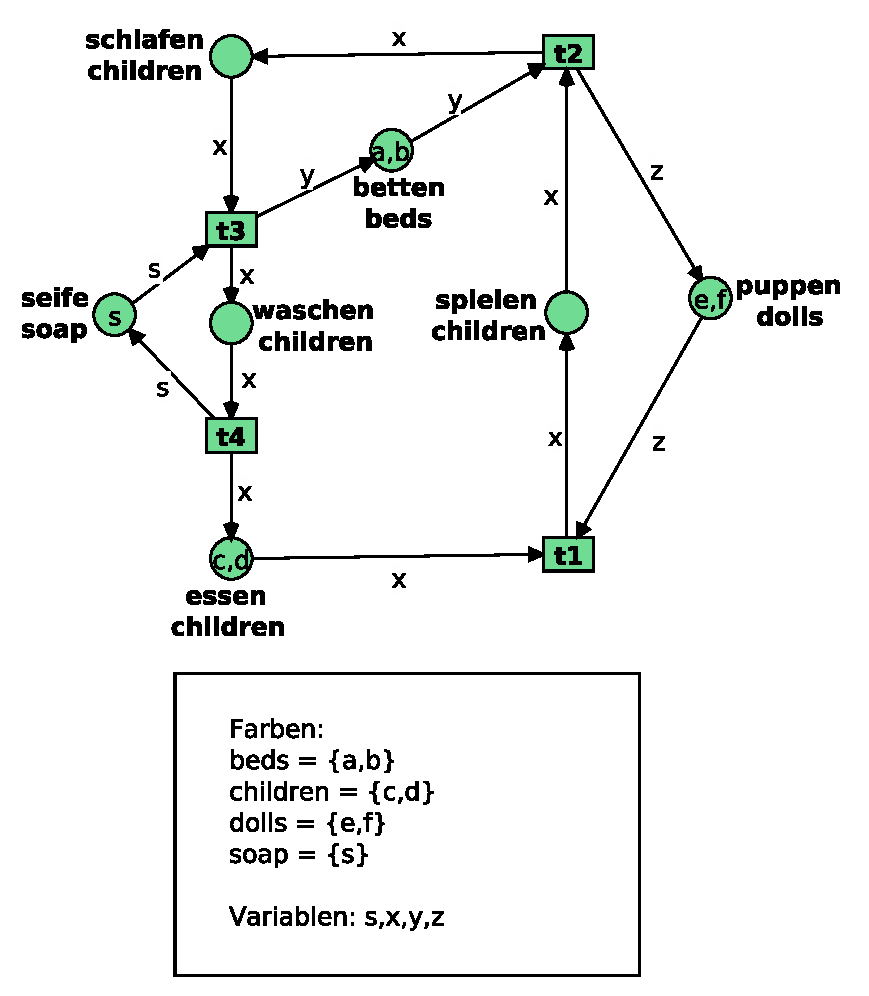
\includegraphics[scale=0.8]{folded.pdf}
\caption{gefärbtes Netz $N_{10.5}$}

\end{figure}

\subsection*{2.}
\subsection*{3.}

\section*{Aufgabe 10.6}
\begin{itemize}
	\item Ein Netz ohne \(\underline{\qquad}\) hei{\ss}t lebendig.\\
		L\"osung: partielle Verklemmungen\\
		\textit{(Lesestoff Woche 10, Teil 1)}
	\item \textit{Flexible Arcs} erlauben das Bewegen von mehreren Marken.\\
		Wahr oder falsch?\\
		\textit{(Lesestoff Woche 10, Teil 2)}
\end{itemize}

\end{document}
